A block diagram of the system model is shown in Fig. \ref{fig:sys_bd}. In this downlink MU-MIMO system, an access point (AP) with $N$ antennas, depicted in the left-hand side of the figure, transmits to $K$ single-antenna stations (STAs), shown on the right-hand side of the figure. The system shown in Fig. \ref{fig:sys_bd} makes use of space division multiple access (SDMA). Each of the $K$ STAs receives its own stream of symbols. The symbols for $STA_i,\ i\in 1,2\ldots,K$ is given as $s_i$. The expected value of the symbol energy is assumed to be normalized to unit power, that is $E \lbrace \vert s_i \vert^2 \rbrace = 1$. 

Before transmission at the AP, each of the $K$ symbols is linearly scaled by a beamforming vector, $\underline w_i$. A maximum ratio transmission (MRT) beamforming scheme is assumed for determining the values of beamforming vectors. Details surrounding of beamforming vector values are discussed in Section \ref{sec:mrt_linear_sinr}, \ref{sec:mrt_wl_sinr}. The power of $\underline w_i$, $\Vert w_i \Vert^2$, is given by the scalar $P_i$, that is: $P_i = \Vert \underline w_i \Vert^2$. The direction of the beamforming vector is given by $\Tilde{\underline w_i}=\frac{\underline w_i}{\Vert \underline w_i \Vert}$. Since $s_i$ is normalized to unit power, the total transmit power at the transmitter is equal to the sum of the beamforming vector powers:
  \begin{equation}
     \begin{aligned}\label{eq:total_power_sum}
     P_{tot} = \sum_{i=1}^K P_i
     \end{aligned}
 \end{equation}


Each of the $K$-$N \times 1$ vectors are summed together and transmitted over a wireless channel $\underline h_i,\ i= 1,2\ldots K$ to the STAs, where $\underline h_i\ \in \mathbb{C}^{1 \times N}$. A Rayleigh fading channel is assumed. Therefore each term in the channel vector $h_i$ follows a complex circularly symmetric iid normal distribution $\mathcal{N}_c(0,\frac{1}{N})$. It follows that the channel norm $\Vert \underline h_i \Vert^2$ follows a gamma distribution with the following parameters: $\Vert \underline h_i \Vert^2 \sim \mathcal{G}(2N,\frac{2}{N})$.

Additive white Gaussian noise (AWGN) is also assumed as shown in Fig. \ref{fig:sys_bd}. The AWGN $n_i$ is assumed to follow a complex circularly symmetric normal distribution, that is: $n_i \sim \mathcal{N}_c(0,\sigma_n^2)$ and $E \lbrace n_j^* n_i \rbrace\ = 0\ \forall i \neq j,\ i,j=1,2,\ldots K$.

The received signal for $STA_i,\ i=1,2\ldots K$, $r_i$, is given by
 \begin{equation}
     \begin{aligned}\label{eq:rx_sig}
        r_i = \underline{h_i}^H \big( \sum_{j=1}^K \underline{w_j}s_j \big) + n_i
     \end{aligned}
 \end{equation}
 This expression can be expanded into a sum of signal, interference, and noise terms.
  \begin{equation}
     \begin{aligned}\label{eq:rx_sig_expanded}
        r_i = \underline{h_i}^H \underline w_i s_i \ +\ \underline{h_i}^H\big( \sum_{j \neq i}^K \underline{w_j}s_j \big)\ +\ n_i
     \end{aligned}
 \end{equation}


\begin{figure}
    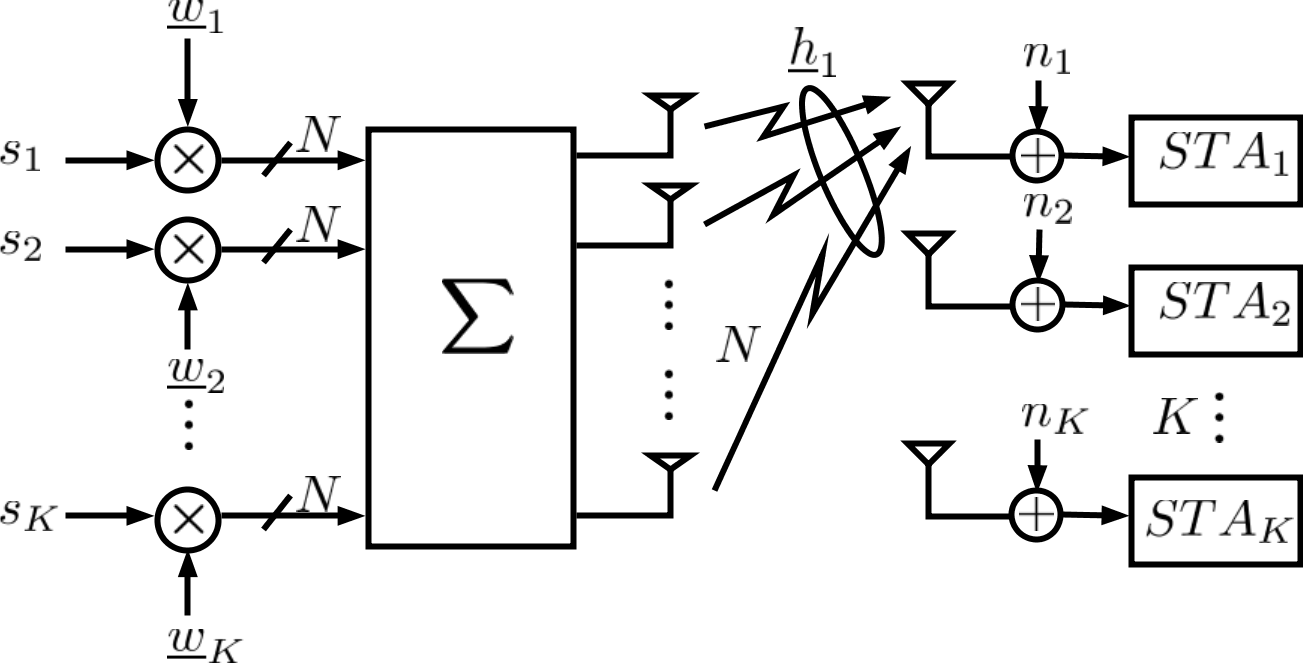
\includegraphics[width=14cm]{figs/system_desc.png}\\
    \caption{Block diagram of the system model.}
    \label{fig:sys_bd}
\end{figure}
